\part{Neural Networks}
%%%%%%%%%%%%%%%%%%%%%%%%%%%%%%%%%%%%%%%%%%%%%%%%%%%%%%%%%%%%%%%%%%%%%%%%%
% Intel Neural Compute Stick 2                                          %
%%%%%%%%%%%%%%%%%%%%%%%%%%%%%%%%%%%%%%%%%%%%%%%%%%%%%%%%%%%%%%%%%%%%%%%%%
\section{Motivation and background}
The motivation of this project is a logical continuation of Part \ref{part:rscam} with the Intel Realsense Camera. In the previous project, a Hardkernel Odroid XU4 (hereafter Odroid) was used because it is comparatively cheaper than existing hardware used for Surewash products. The issue with Odroid is that it is still comparatively expensive in comparison to a Raspberry Pi (a casual search on Amazon suggests that it is at least 3-4 times more expensive). The issue with the Raspberry Pi is that its hardware is not capable of running the Surewash algorithm in a time critical setting, which is of course needed, since one of the key selling points of Surewash is that it can give live feedback to the user. A potential solution to this problem is using an Intel Neural Compute Stick, hereafter NCS. This is a low-power device that can interface with a Raspberry Pi via the USB protocol. The cornerstone of the NCS is the Myriad chip.

The Myriad chip is described by Intel as a `Vision Processing Unit', hereafter VPU (not to be confused with a Video Processing Unit). One might already be familiar with the concept of a CPU, or Central Processing Unit, which is a microchip designed for general purpose computing, and a GPU, or Graphics Processing Unit, which is specifically optimised for {\slshape embarrassingly parallel} calculations, such as graphics processing, hence the name. The VPU is similar in idea to a GPU in that it is optimised for parallel computing, except that it is specifically designed for low-power situations (\cite{7024073}), and it is particularly suited for inferring convolutional and fully-connected artificial neural networks on mobile devices (inferring an artificial neural network means simply to evaluate it, distinct from training it).

The current Surewash algorithm uses traditional computer vision methods which are not well suited for a device like the NCS, and so the algorithm for processing hand gestures will have to be rethought in order to work on the NCS.

\section{Underlying concepts}
    \subsection{Graphs}
    A graph is a is a mathematical concept where a series of nodes are connected together by vertices (\cite{chartrand2010graphs}). A classic example of graph theory in the real world is for computer-aided map directions; locations can be nodes, and roads vertices. A computer can give directions based on this graph using {\slshape Dijkstra's Algorithm} (\cite{dijkstra1959note}).

    \begin{figure}[h]
        \centering
        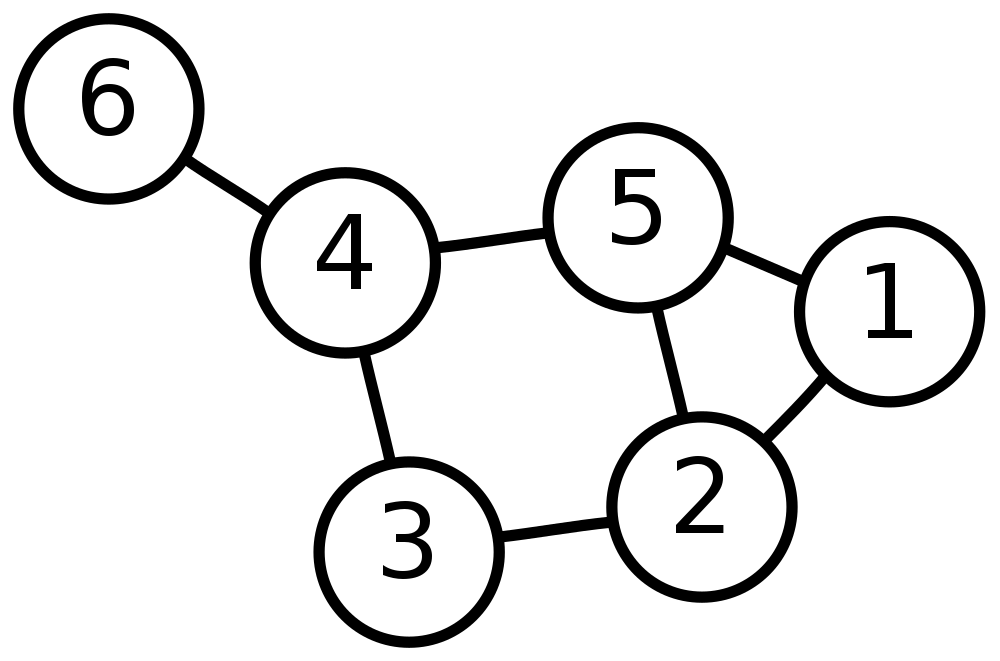
\includegraphics[width=100px]{../img/1000px-6n-graf.png}
        \caption[]{An example graph\footnotemark}
        \label{fig:simplegraph}
    \end{figure}

    \footnotetext{Obtained from: https://commons.wikimedia.org/wiki/File:6n-graf.svg (accessed: 26-05-2019)}

    Figure \ref{fig:simplegraph} is an example of a simple graph. Graphs can be broken down into two broad types: undirected, and directed. In an undirected graph, the vertices are always unidirectional, but in a directed graph, or digraph, each vertex in a graph has a direction associated with it. In a graph, the vertices can also have weights associated with them. For example, in the context of a graph to model a road map, larger weights might denote a longer road, and a smaller weight, a shorter road. The graph is the fundamental building block to Artificial Neural Networks.

    \subsection{Artificial Neural Networks}
    Artificial Neural Networks, hereafter ANNs in essence are graphs. Specifically, ANNs are directed, acyclic, weighted graphs. An acyclic graph is one that has a defined entry and exit point, and no loops within the graph, so the evaluation of the graph is finite. ANN are so-called because they aim to emulate the function of Biological Neural Networks, so each node acts as a `neuron', with defined weighted connections to other neurons \cite{hopfield1982neural}. In a typical ANN, neurons are divided into a sequence of layers starting with the input layer, then one or more `hidden' layers, followed by an output layer. Each neuron in a layer is connected to some or all neurons in the previous layer with weighted vertices, and its output is the sum of those weighted vertices passed into some function, called the {\slshape activation function}. 

    \begin{figure}[h]
        \centering
        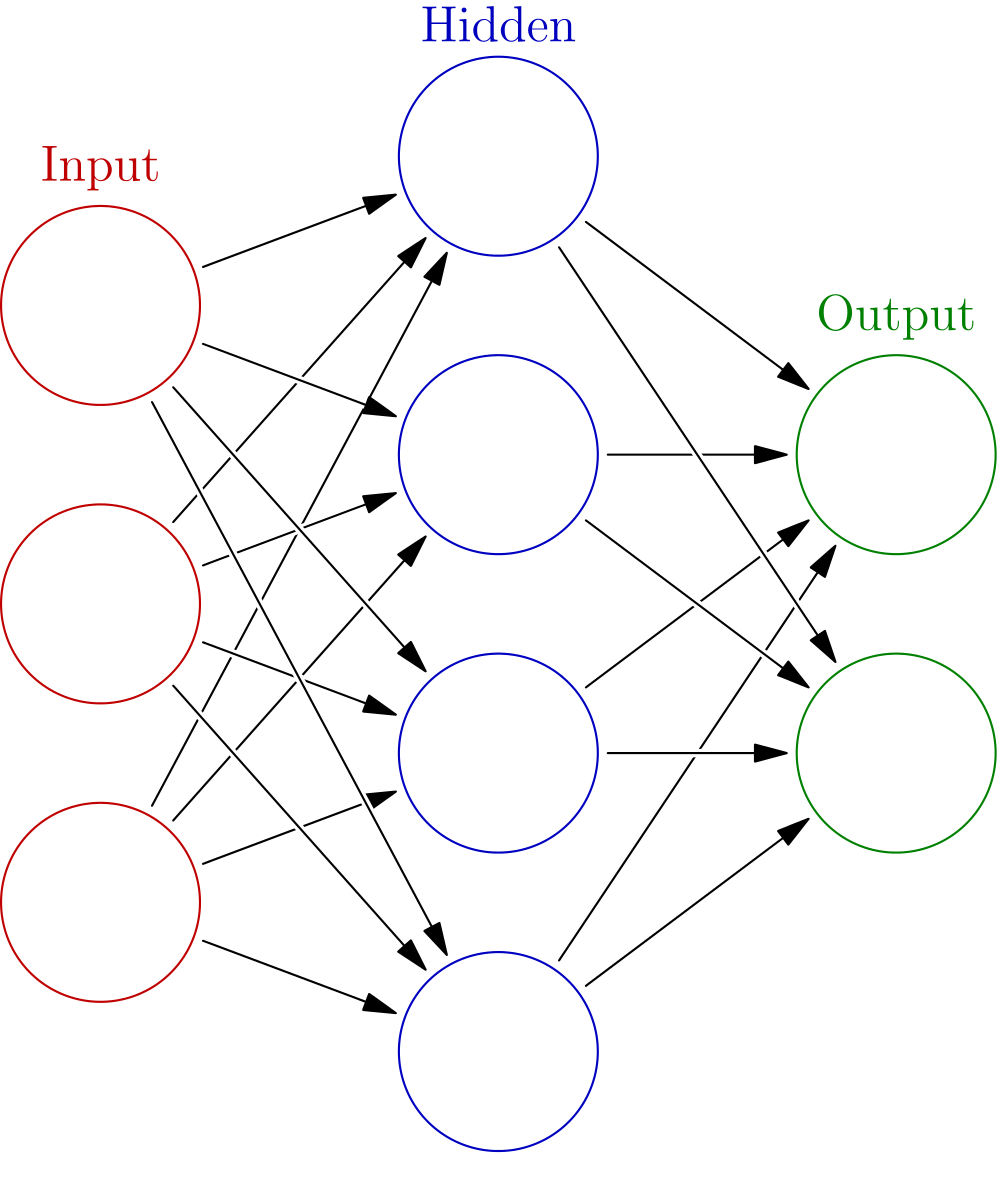
\includegraphics[width=150px]{../img/1000px-Colored_neural_network.png}
        \caption[]{An example ANN\protect\footnotemark}
        \label{fig:fcneuralnet}
    \end{figure}
    
    Figure \ref{fig:fcneuralnet} is an example of a simple neural network (the neurons are `fully connected', so each neuron in a layer is connected to all of the neurons from the previous layer), this graph takes three scalar inputs, and produces two scalar outputs.
    
        \subsubsection{The Neuron}
        Formally, a neuron looks like Figure \ref{fig:theneuron}.
        \begin{figure}[h]
        \[
            u=f(w_0+\sum_{i=1}^nw_ix_i)
        \]
        \caption{The Neuron}
        \label{fig:theneuron}
        \end{figure}
        
        Where $x_i$ represents the input of a previous neuron, or the entry to the graph, $w_i$ represents a weight that $x_i$ is multiplied by, $w_0$ represents the `bias' which is simply a scalar value, and $f$ is some function that produces the scalar output for that neuron.
        
        \subsubsection{Activation Functions}
        Figure \ref{fig:activationeg} shows examples of activation functions that can be used. In this project, ReLU was used primarily.\\
        \footnotetext{Obtained from: https://commons.wikimedia.org/wiki/File:Colored\_neural\_network.svg (accessed: 26-05-2019) }

        \begin{figure}[h]
            \centering

        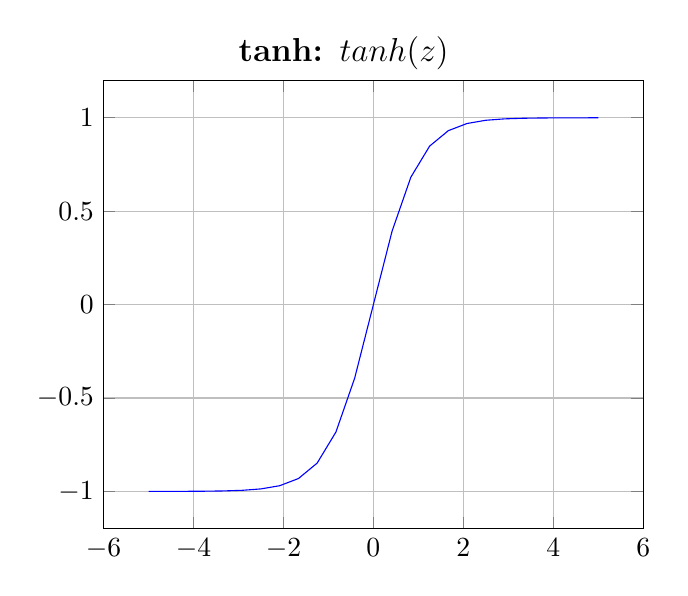
\begin{tikzpicture}
            \begin{axis}[grid=both,
                ]
                \addplot[blue] {tanh(x)};
            \end{axis}
            \node[above,font=\large\bfseries] at (current bounding box.north) {tanh: $tanh(z)$};
        \end{tikzpicture}
        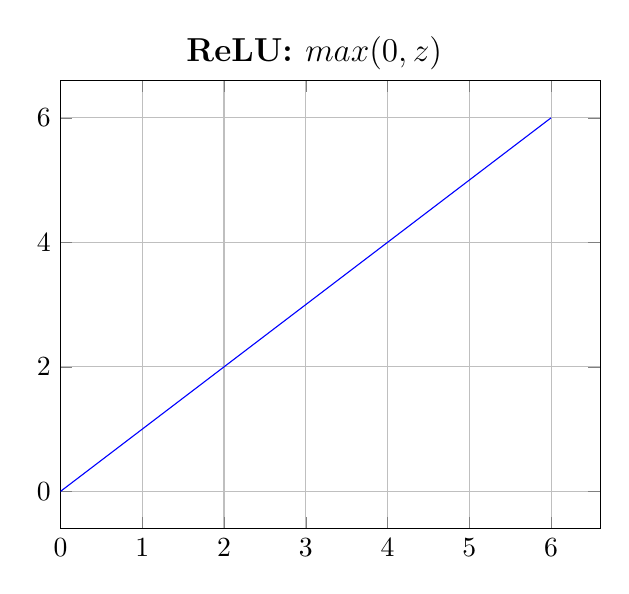
\begin{tikzpicture}
            \begin{axis}[grid=both,xmin=0
                ]
                \addplot+[mark=none,blue,domain=-3:0] {0};
                \addplot+[mark=none,blue,domain=0:6] {x};
            \end{axis}
            \node[above,font=\large\bfseries] at (current bounding box.north) {ReLU: $max(0, z)$};
        \end{tikzpicture}

        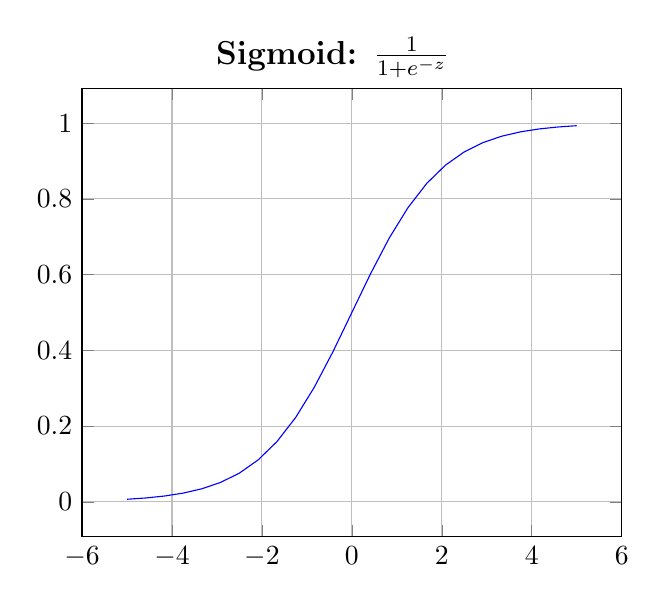
\begin{tikzpicture}
            \begin{axis}[grid=both,
                ]
                \addplot[blue]  {1/(1+exp(-x))} node[above]{};
            \end{axis}
            \node[above,font=\large\bfseries] at (current bounding box.north) {Sigmoid: $\frac{1}{1+e^{-z}}$};
        \end{tikzpicture}
        \caption{Activation function examples}
        \label{fig:activationeg}    
    \end{figure}

          \subsubsection{Training ANNs}
          Once a particular architecture has been decided upon, the next task is to train a neural network. The goal of training a neural network is to find the optimal values for the weights $w_i$ in the neural network. Backpropagation, which in its modern form is described by \cite{rumelhart1988learning} is the predominant algorithm used to optimise the weights.

          In the first stage (the forward pass), the network is evaluated by passing an input through, and the output of the network is passed to a loss function, which will produce a scalar loss value (for a particular input, an particular output is expected, the loss value is some indication of how far off the predicted value is over the actual value). In the second stage (the backward pass), the network is evaluated in reverse, going through each layer, the partial derivative (i.e. the gradient) of each neuron's output is evaluated using the chain rule. The weights for each neuron can then be adjusted using gradient descent, see Figure \ref{fig:gradientdescent} (where $\mu$ is the learning rate). The learning rate is typically set for all of the neurons, an example value might be 0.1, and this can be programmatically adjusted during training, see \cite{learningratetypes}.

          \begin{figure}[h]
            \[
                w_{n+1}=w_n-\mu \frac{d}{dw}f(w_0+\sum_{i=1}^nw_ix_i)
            \]
            \caption{Gradient Descent}
            \label{fig:gradientdescent}
            \end{figure}

\section{Workflow}
    \subsection{Hardware}
    Training a neural network is not a trivial task computationally speaking. The computer that I work with, by today's standards has a high specification, but it is wholly inadequate for training neural networks, which is due to the nature of how neural networks are trained. Graphics Processing Units, or GPUs have been shown to be quicker at training neural networks (\cite{OH20041311}). Since there was no adequate GPU readily available at work, I set up an AWS (Amazon Web Services) instance which had a GPU. I did have to be conscious of cost, since the server cost circa USD\$0.80 per hour and my budget was limited. As an example of the difference that using AWS makes, I compared training the same neural network on my computer, and on the AWS server, to train one epoch on my own computer took approximately 60 minutes, but only took 2 minutes on the AWS server.

    Any work that did not involve training neural networks was completed on my own computer.

    \subsection{Software}
        \subsubsection{Programming Language}
        Most data processing was done with the Intel distribution of Python (my own computer has an Intel Coffee Lake CPU) since it is compiled to take advantage of special Intel CPU instructions for vector manipulation. Some miscellaneous work was also done with Bash script.

        \subsubsection{ANN Training}
        For designing and training the neural networks, I used Keras (\cite{chollet2015keras}) because I had used it before. Keras is a high-level Python framework for designing ANNs, and acts as a frontend for other ANN frameworks, I chose Tensorflow (\cite{tensorflow2015-whitepaper}) as the backend because it is compatible with the NCS, and it is also relatively ubiquitous among the deep learning community.

        \subsubsection{Miscellaneous Processing}
        NumPy (\cite{5725236}) is a Python library for fast matrix multiplication. Since Python is a scripted language, vector and matrix operations are slow in native code, so NumPy can process these operations faster.

        When uploading data to the AWS server, I used 7-Zip for file compression since the file size was usually large (4.32GB as one example was reduced to 699MB), and it took considerable time to upload large files like this.


\section{Data}
    \subsection{Introduction}
    As of writing this, it is still something of an open question as to how much data is required to effectively train a neural network, one of the key challenges with this project is acquiring enough data. When I started the project, I was given a labelled dataset containing 5114 images of hands, which is certainly too small, when ANNs such as VGG16 (\cite{vggnet}) were trained on many multiples the size of the dataset that I was given. The simplest strategy is to acquire more data, but without a defined procedure in place, this can be a time consuming, and costly process. Another strategy to get around limited data is employ data augmentation strategies, such as rotations, affine transformations, and background modification.

    \subsection{Data Acquisition}
    acquiring more data is the best way to overcome a small dataset, but the acquisition process needs to be streamlined in order to achieve this task effectively. This was forked into a separate project which is described in the next part.

    \subsection{Data Augmentation}
        \subsubsection{Backgrounds}
        The background for the images in dataset given was a white sheet, so if the ANN was trained on just this, it is unlikely to work with any other type of background. My strategy to ensure that the ANN learns to ignore the background, is inputting images of hands among a diverse range of backgrounds. A convenient aspect of the data that I was given was that each image of a hand pose contained a corresponding binary image separating foreground and background pixels, it is therefore a trivial task to replace the background of these images. The logic in Figure \ref{fig:handlogic} was used, Figure \ref{fig:handlogicimg} shows a visualisation of the process.
        
        \begin{figure}
            \centering
        % \begin{gather*}
        $Y_{foreground} = HAND \land ROI$ \\
        $Y_{background} = BACKGROUND \land \lnot ROI$\\
        $OUTPUT = Y_{background} \lor Y_{foreground}$
        % \end{gather*}
        \caption{Background Replacement}
        \label{fig:handlogic}
    \end{figure}

        \begin{figure}[h]
            \centering
            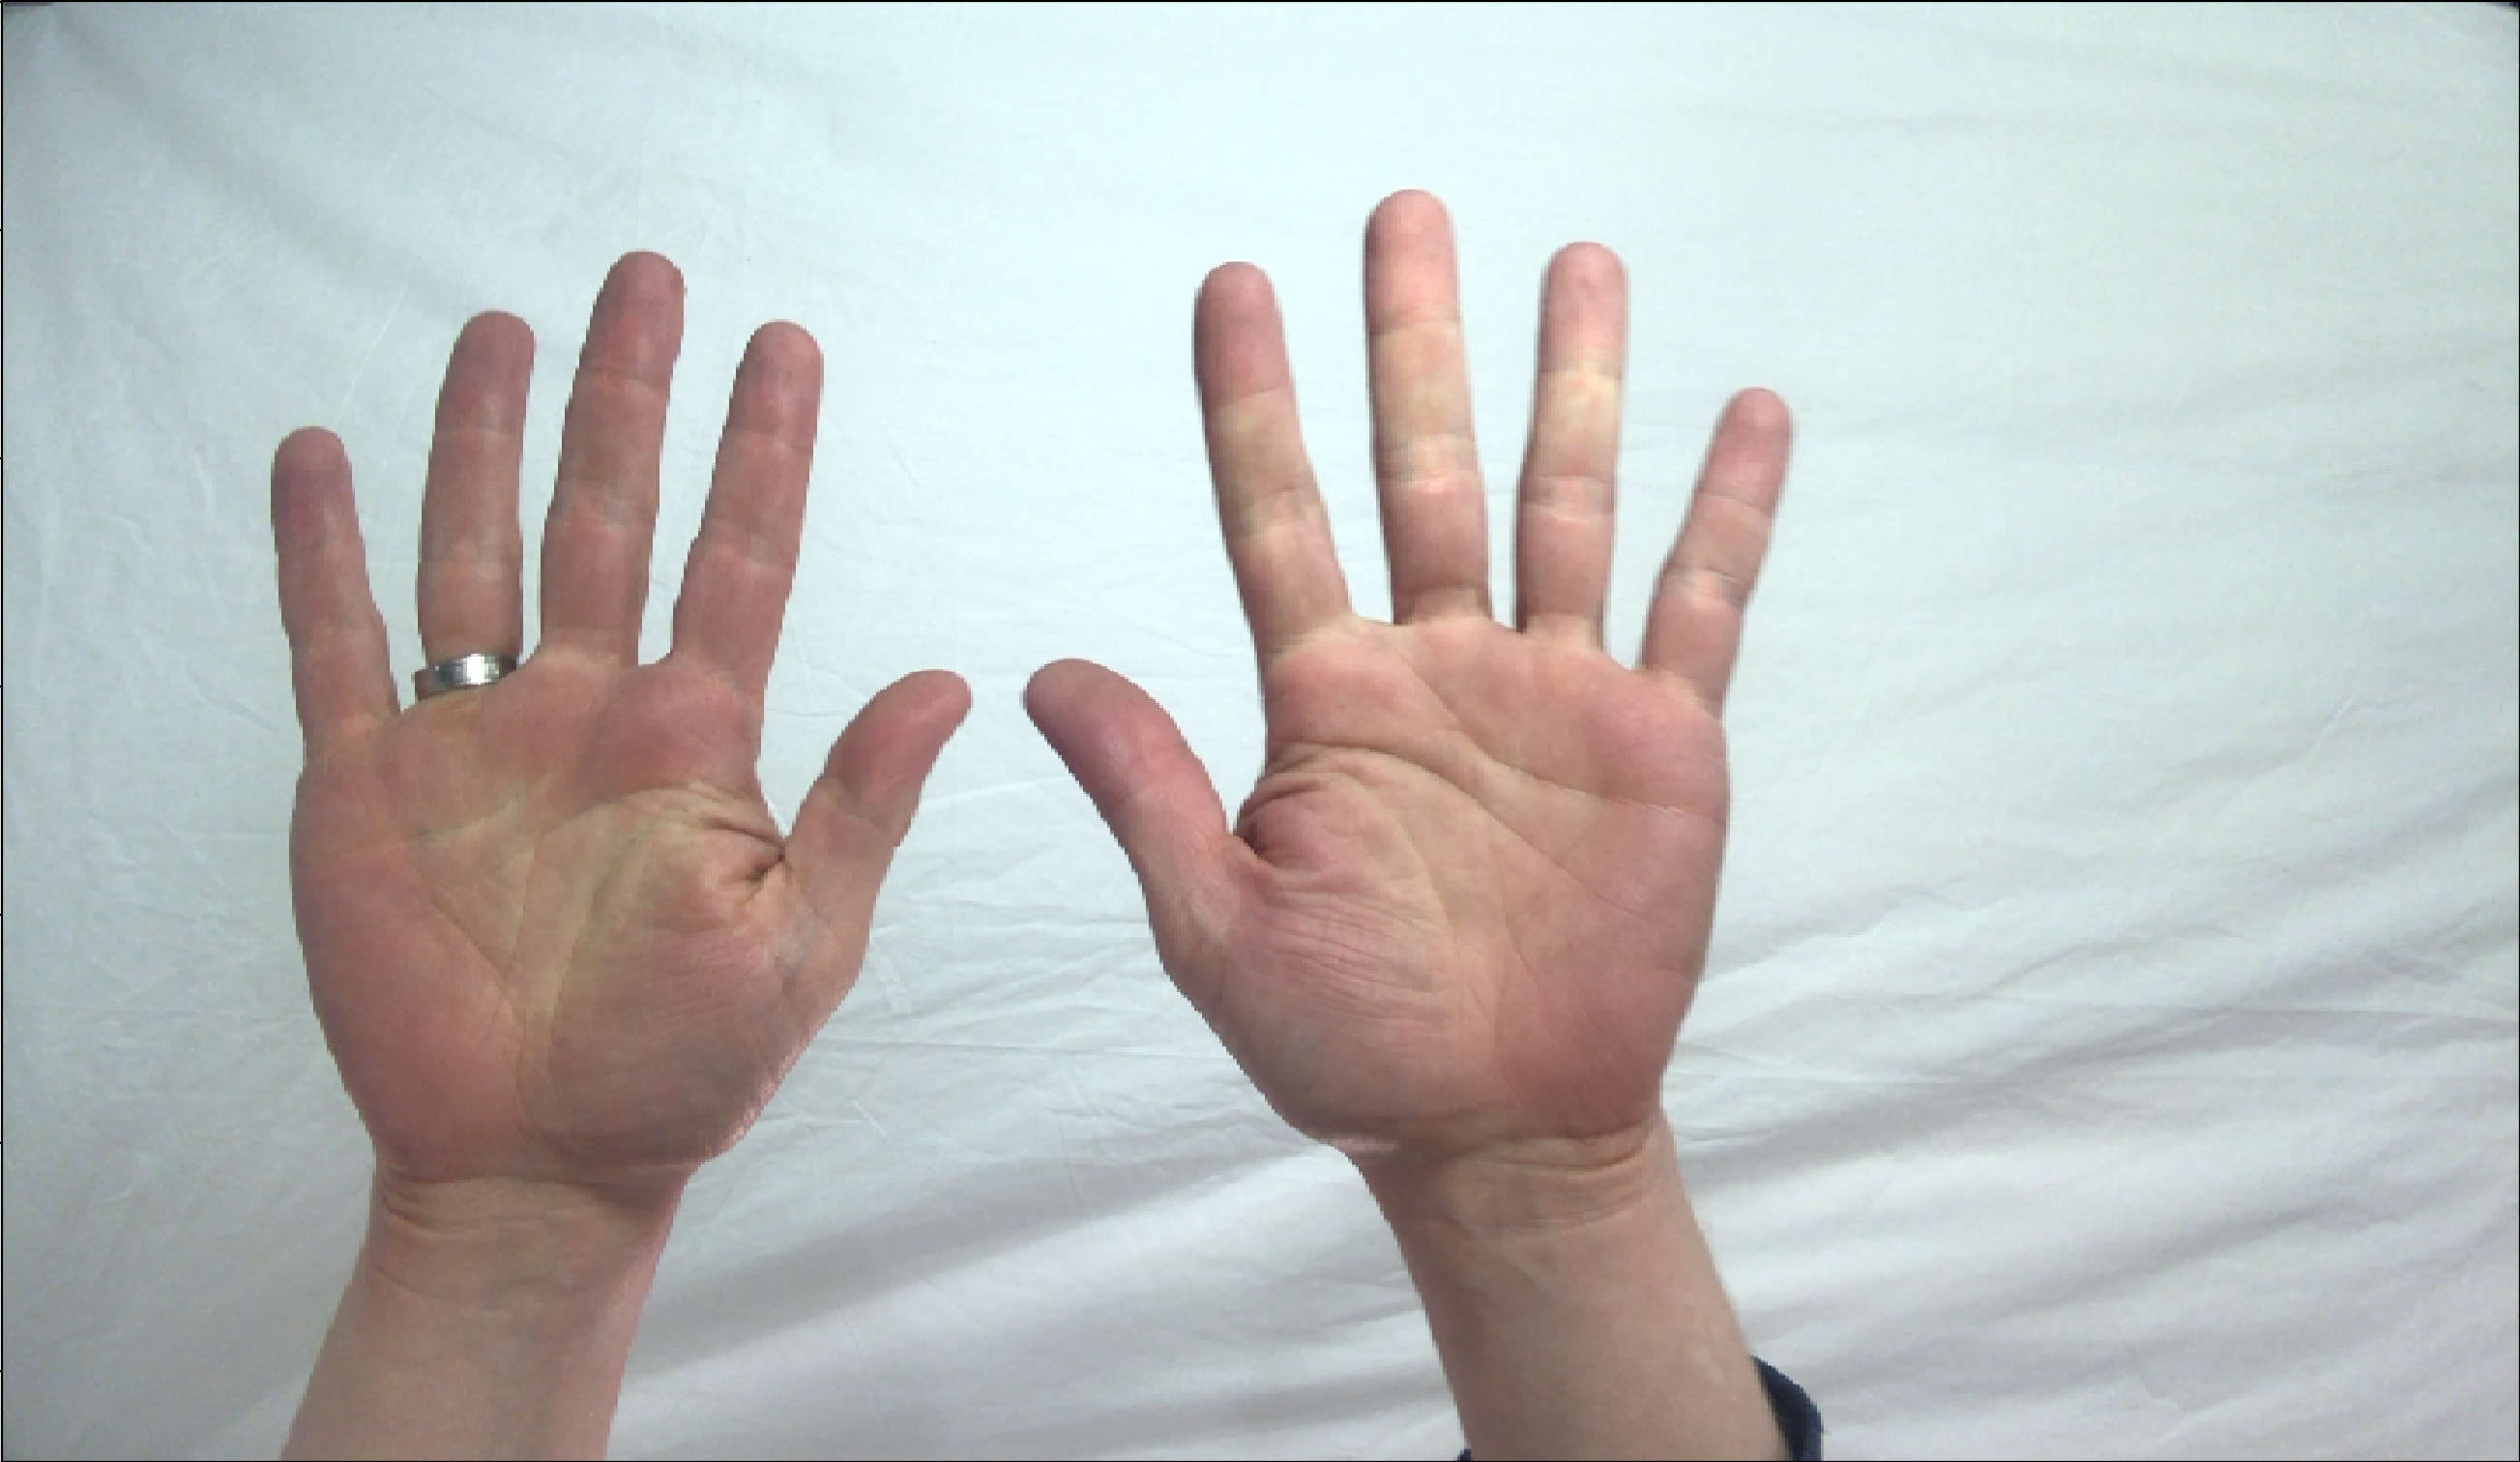
\includegraphics[width=114pt]{../img/handspipeline/1.png}
            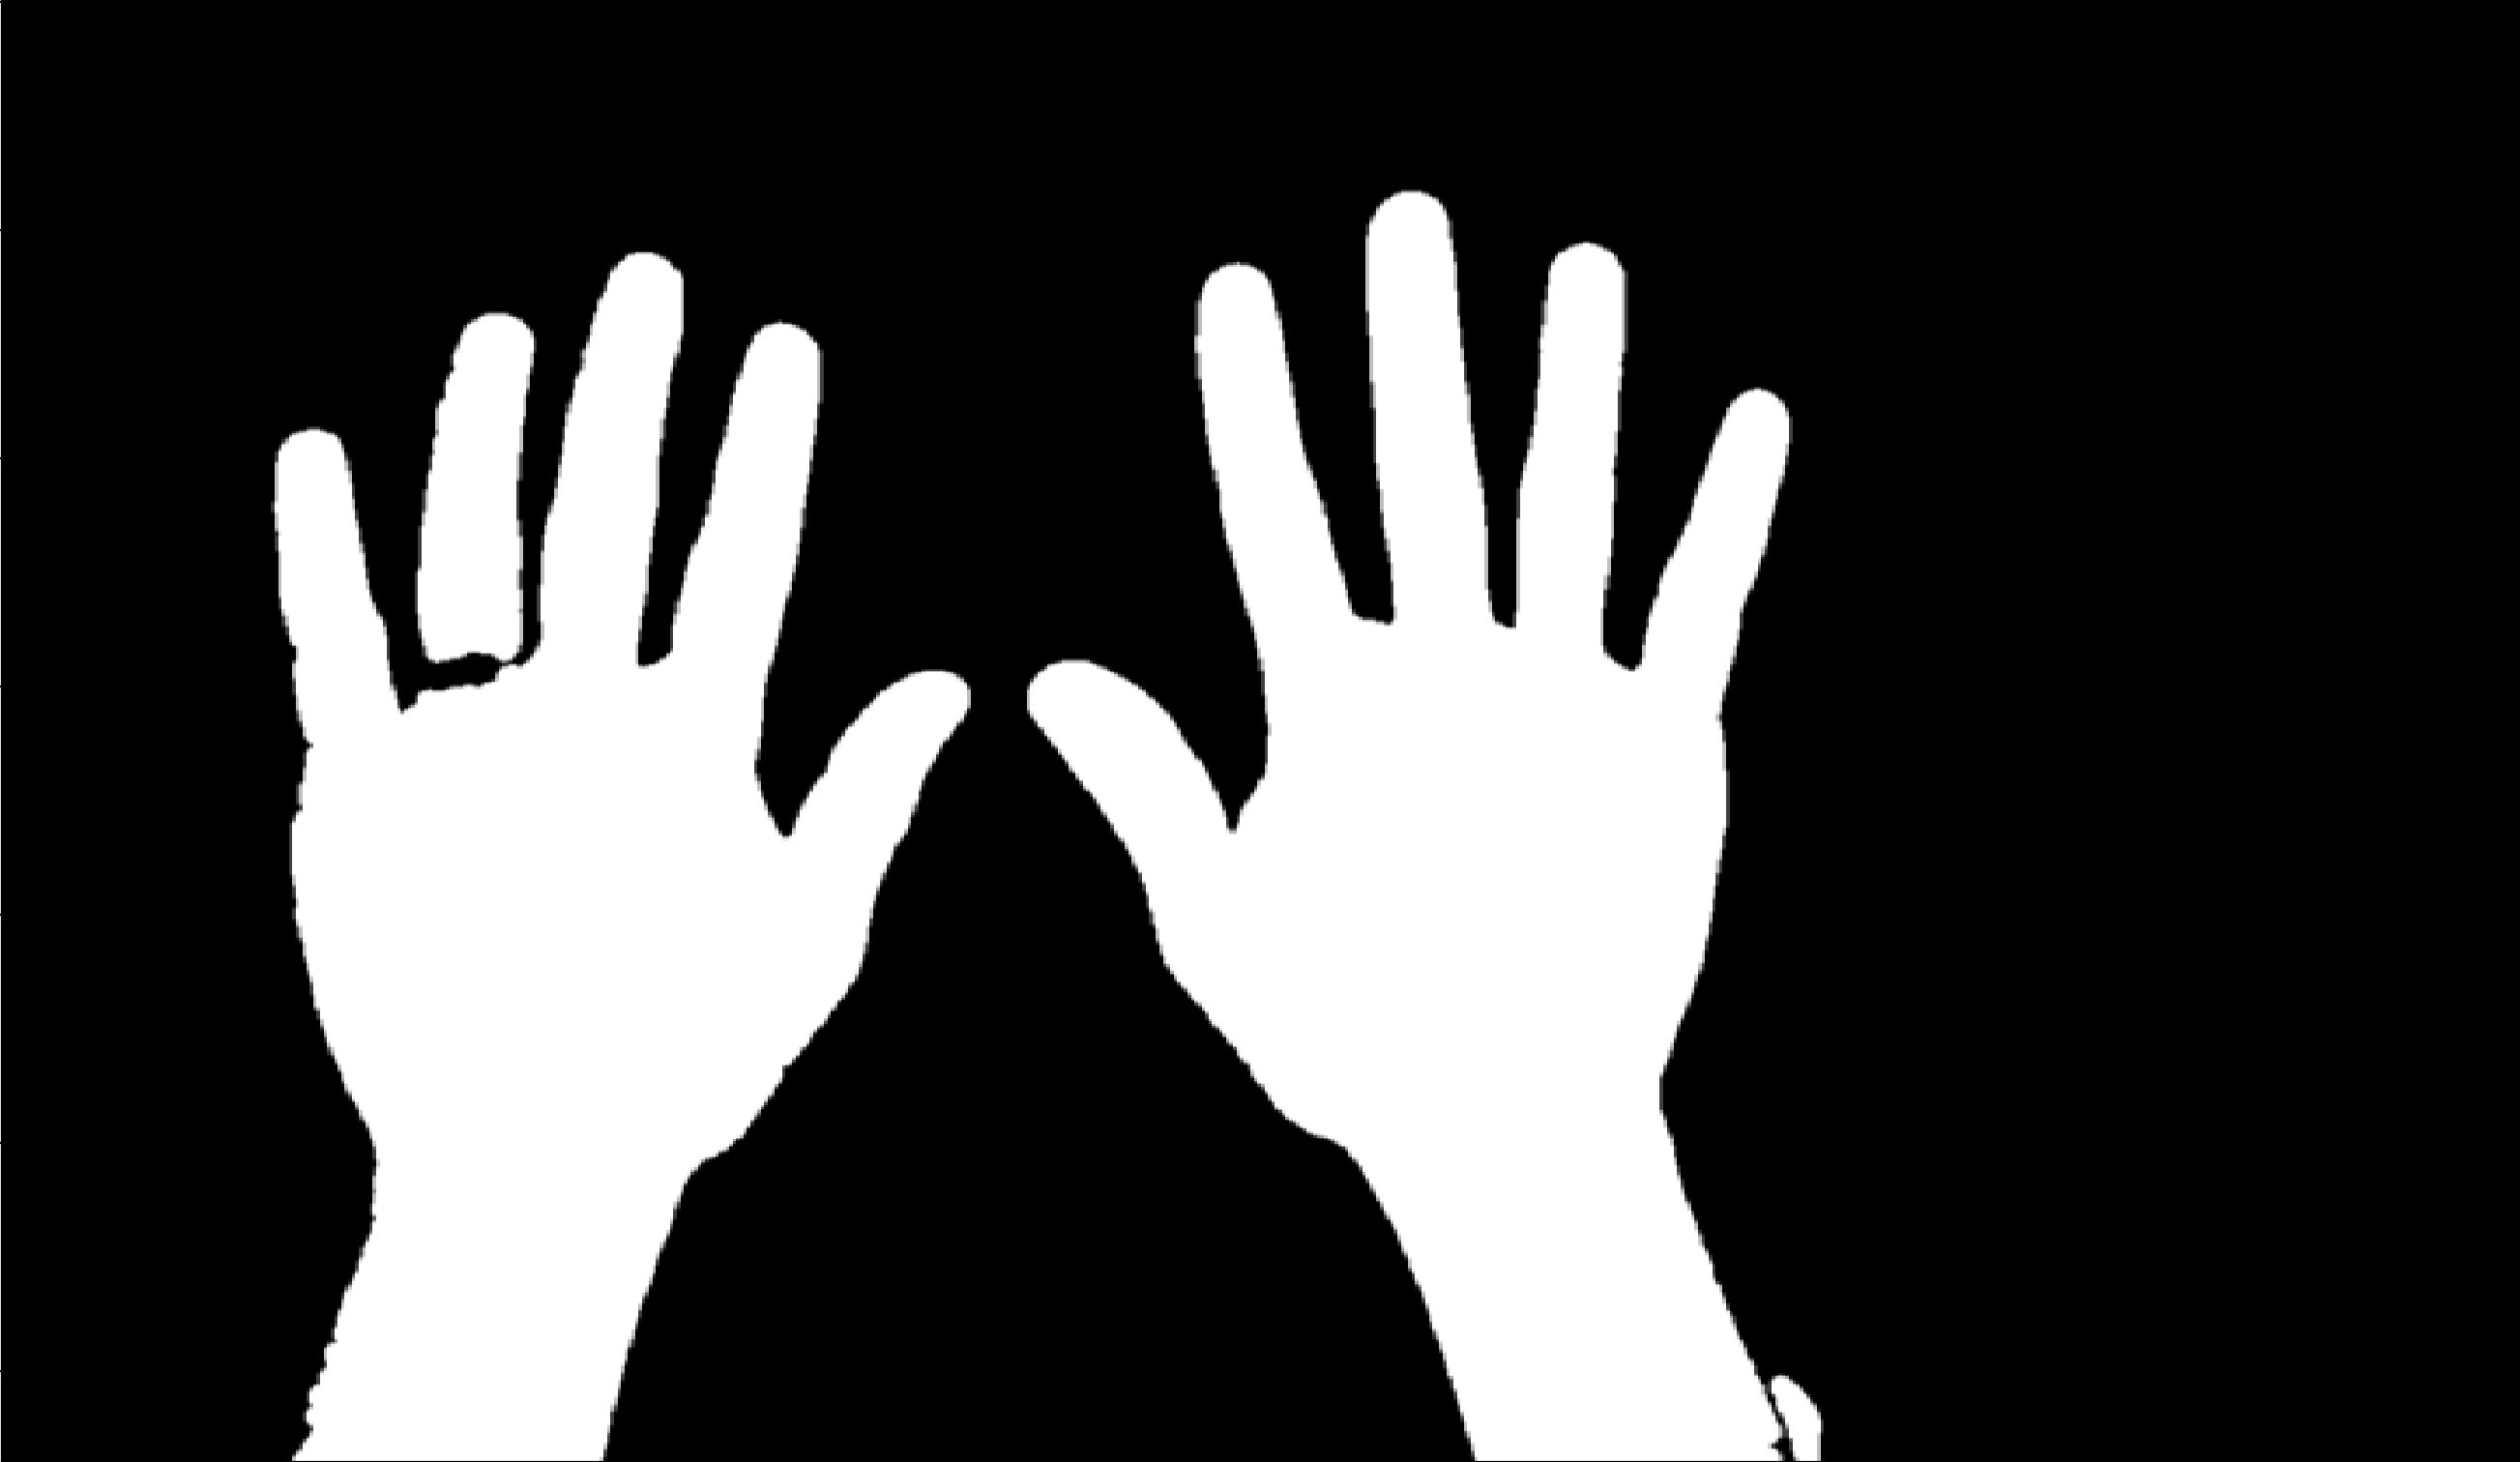
\includegraphics[width=114pt]{../img/handspipeline/2.png}
            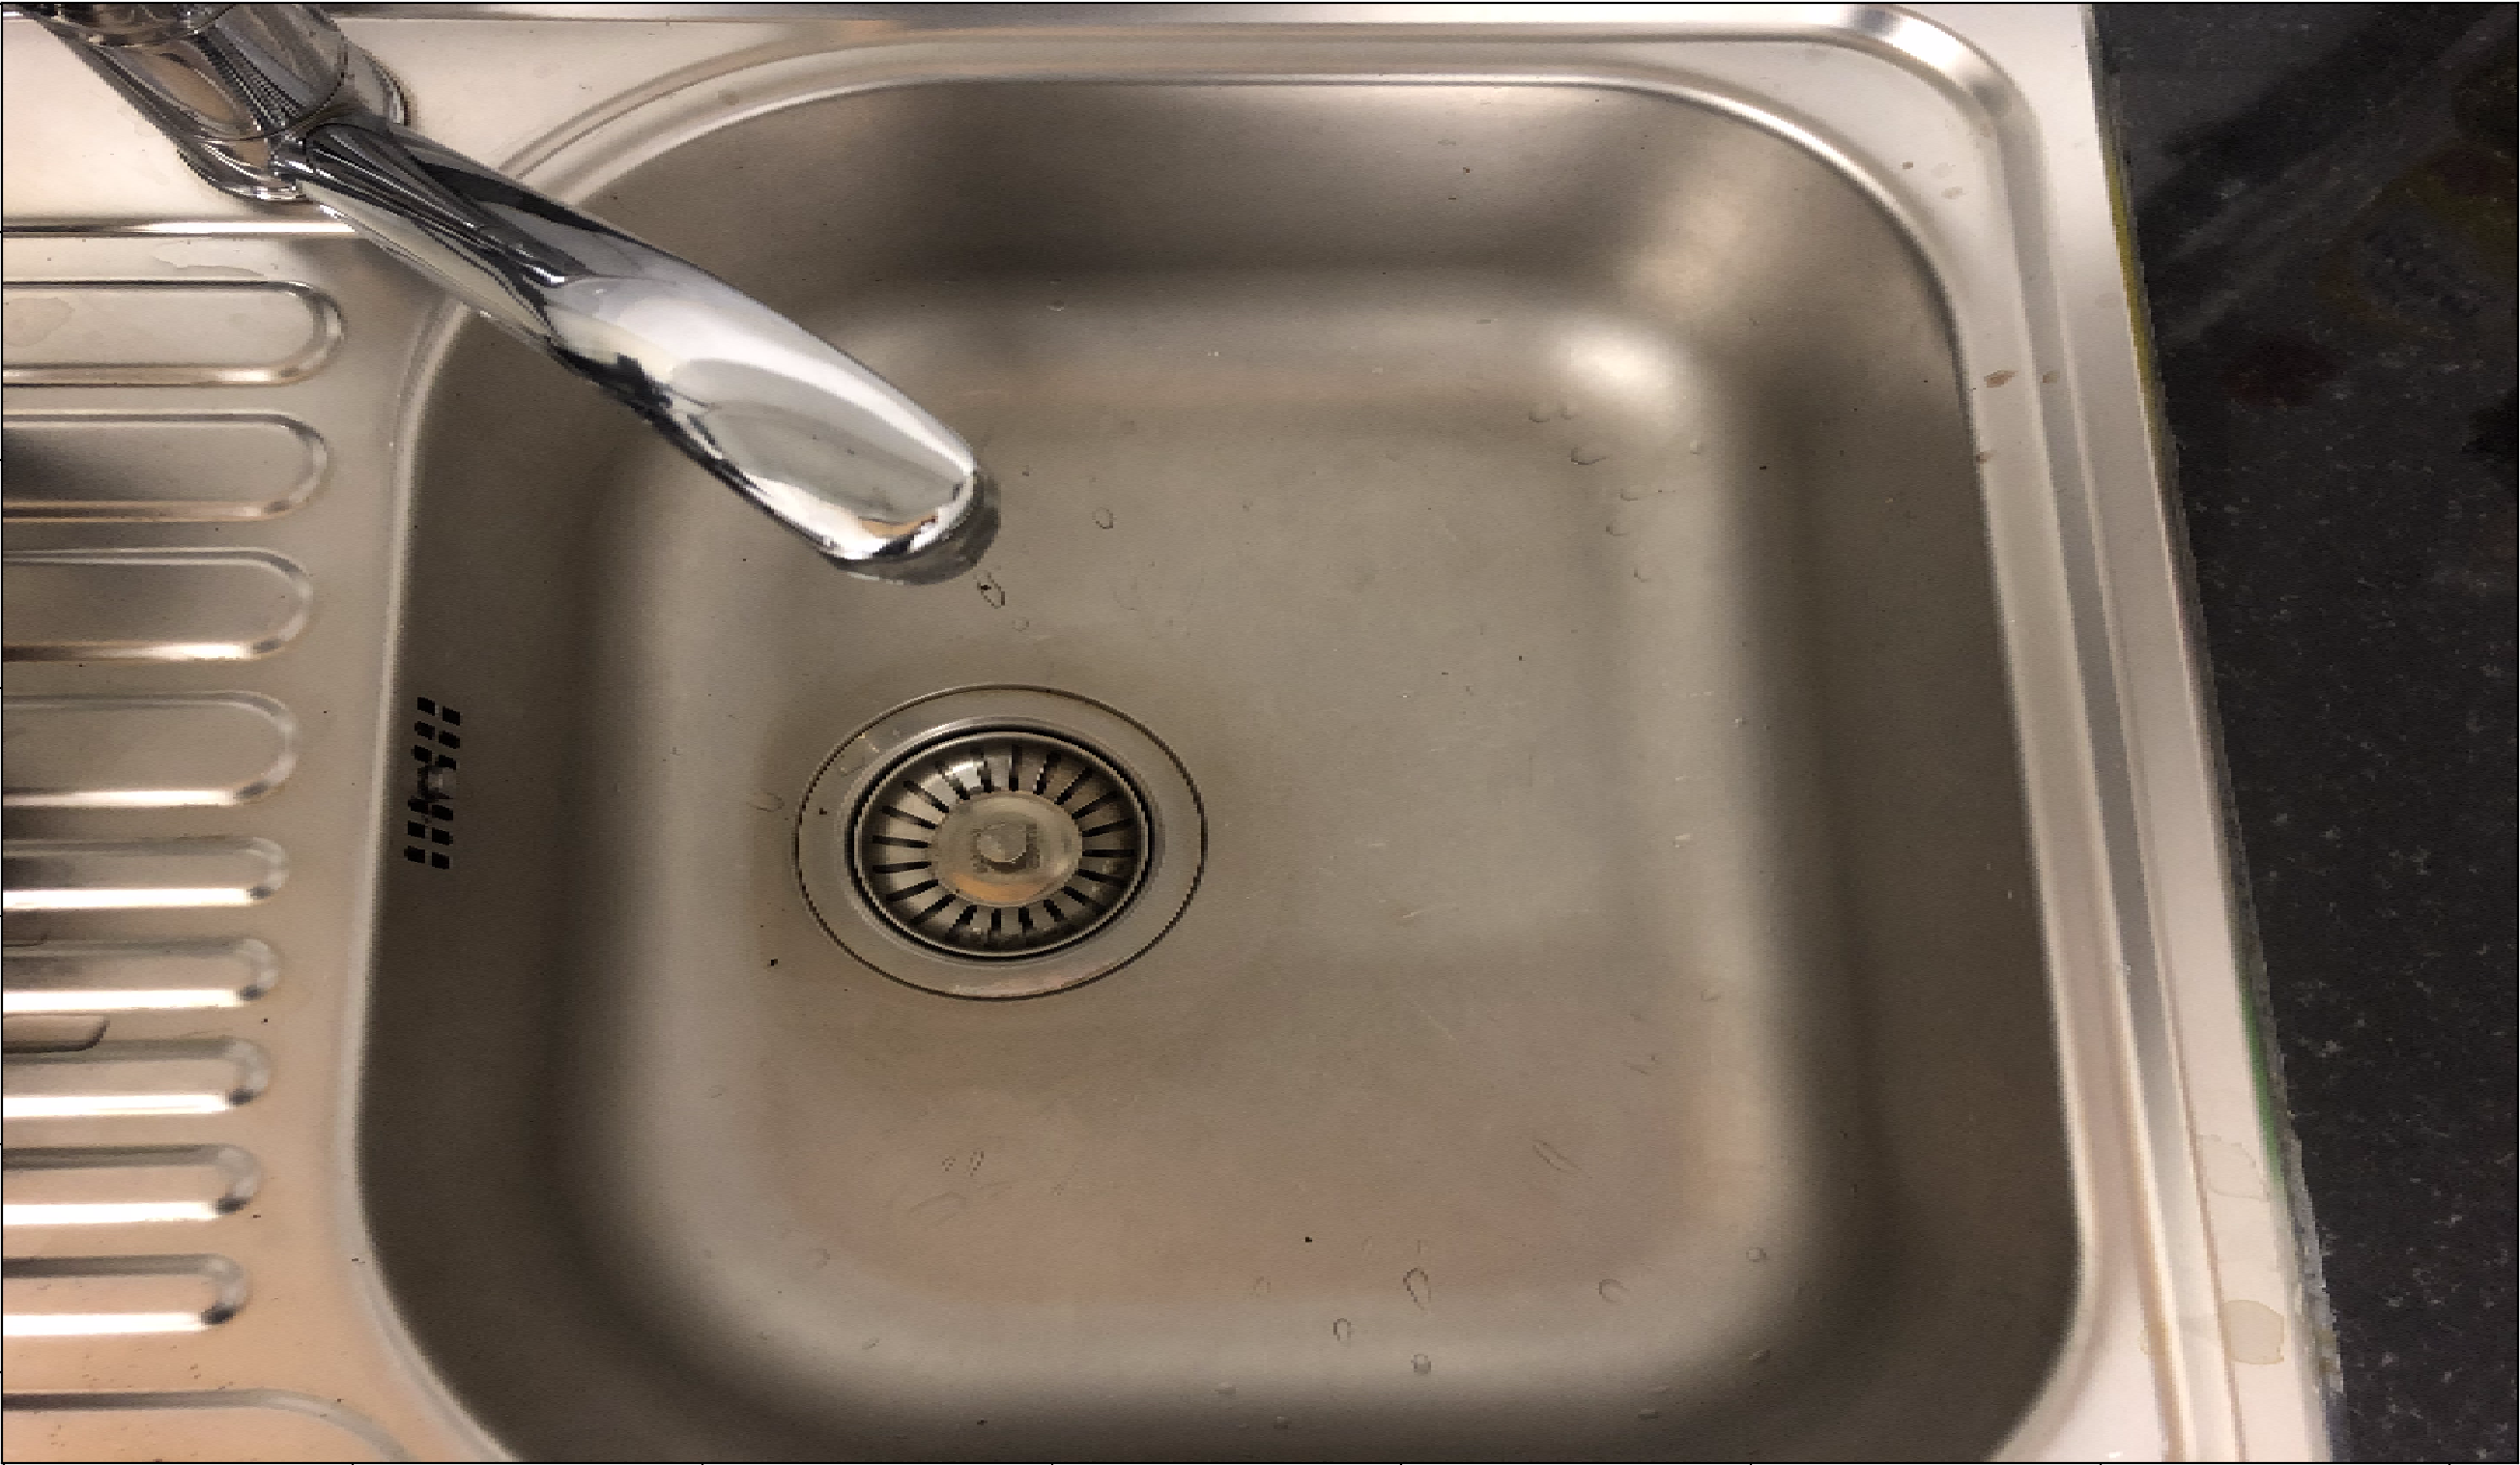
\includegraphics[width=114pt]{../img/handspipeline/3.png}\\
            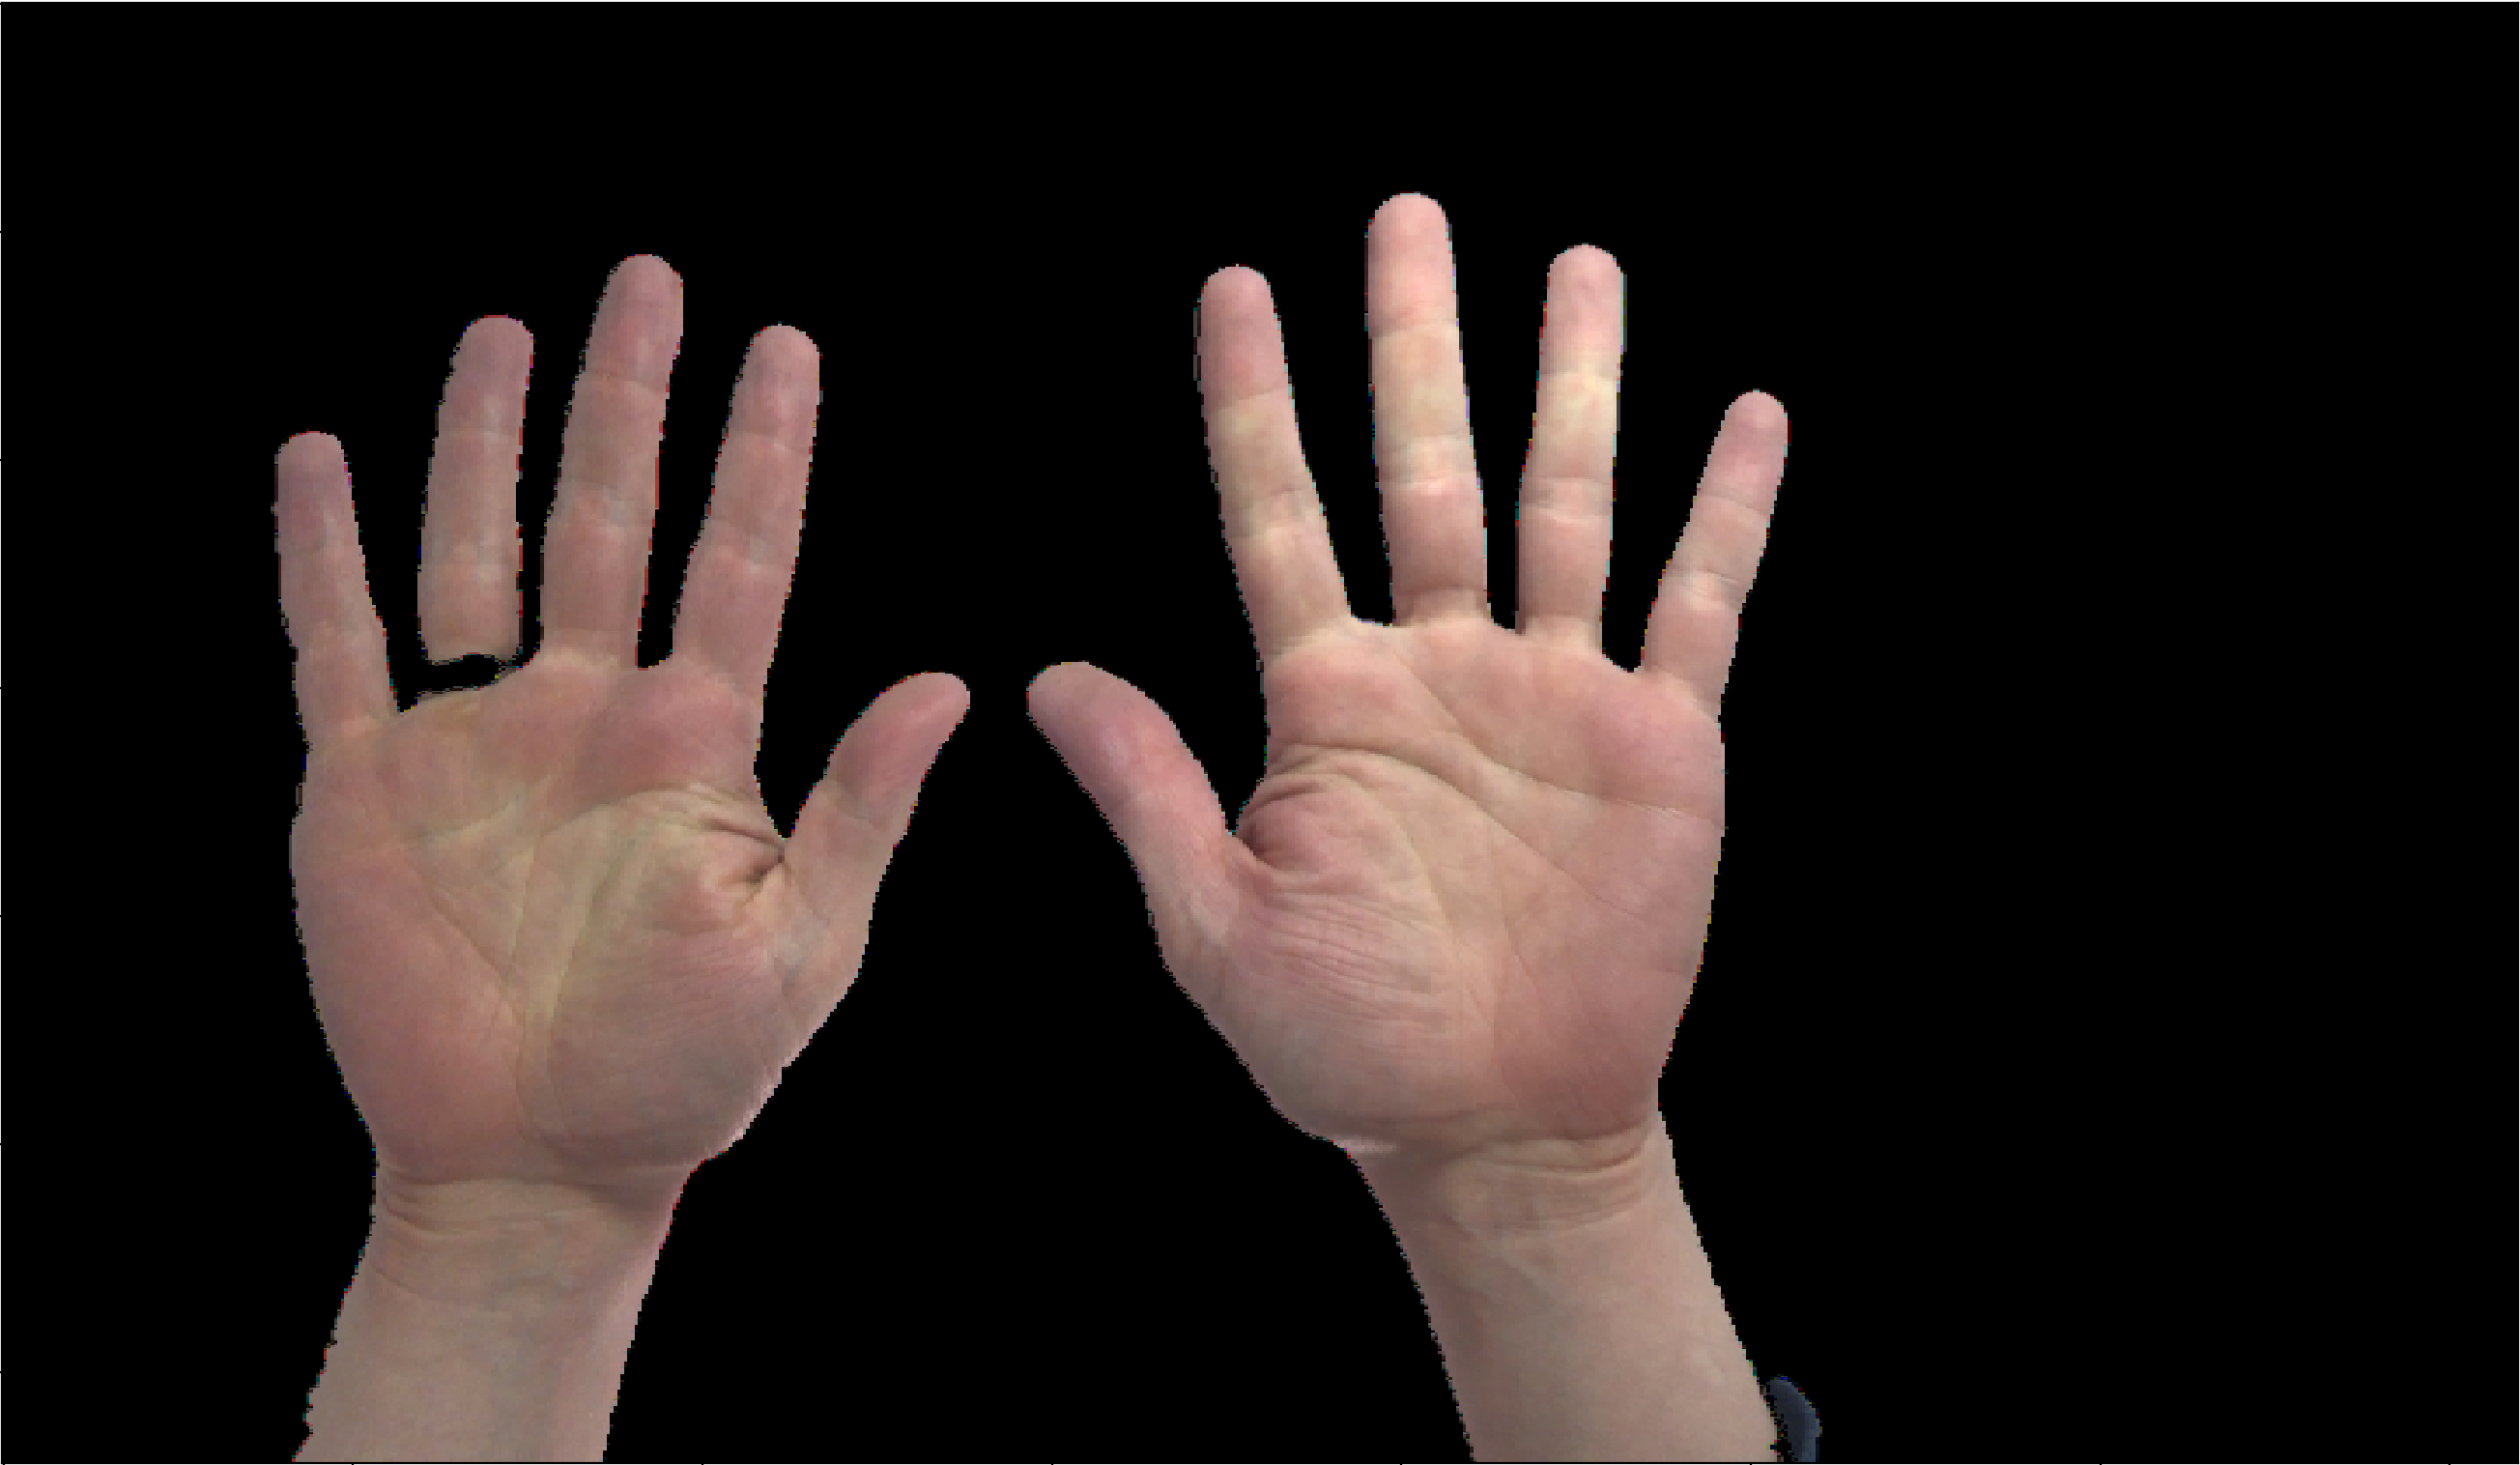
\includegraphics[width=114pt]{../img/handspipeline/4.png}
            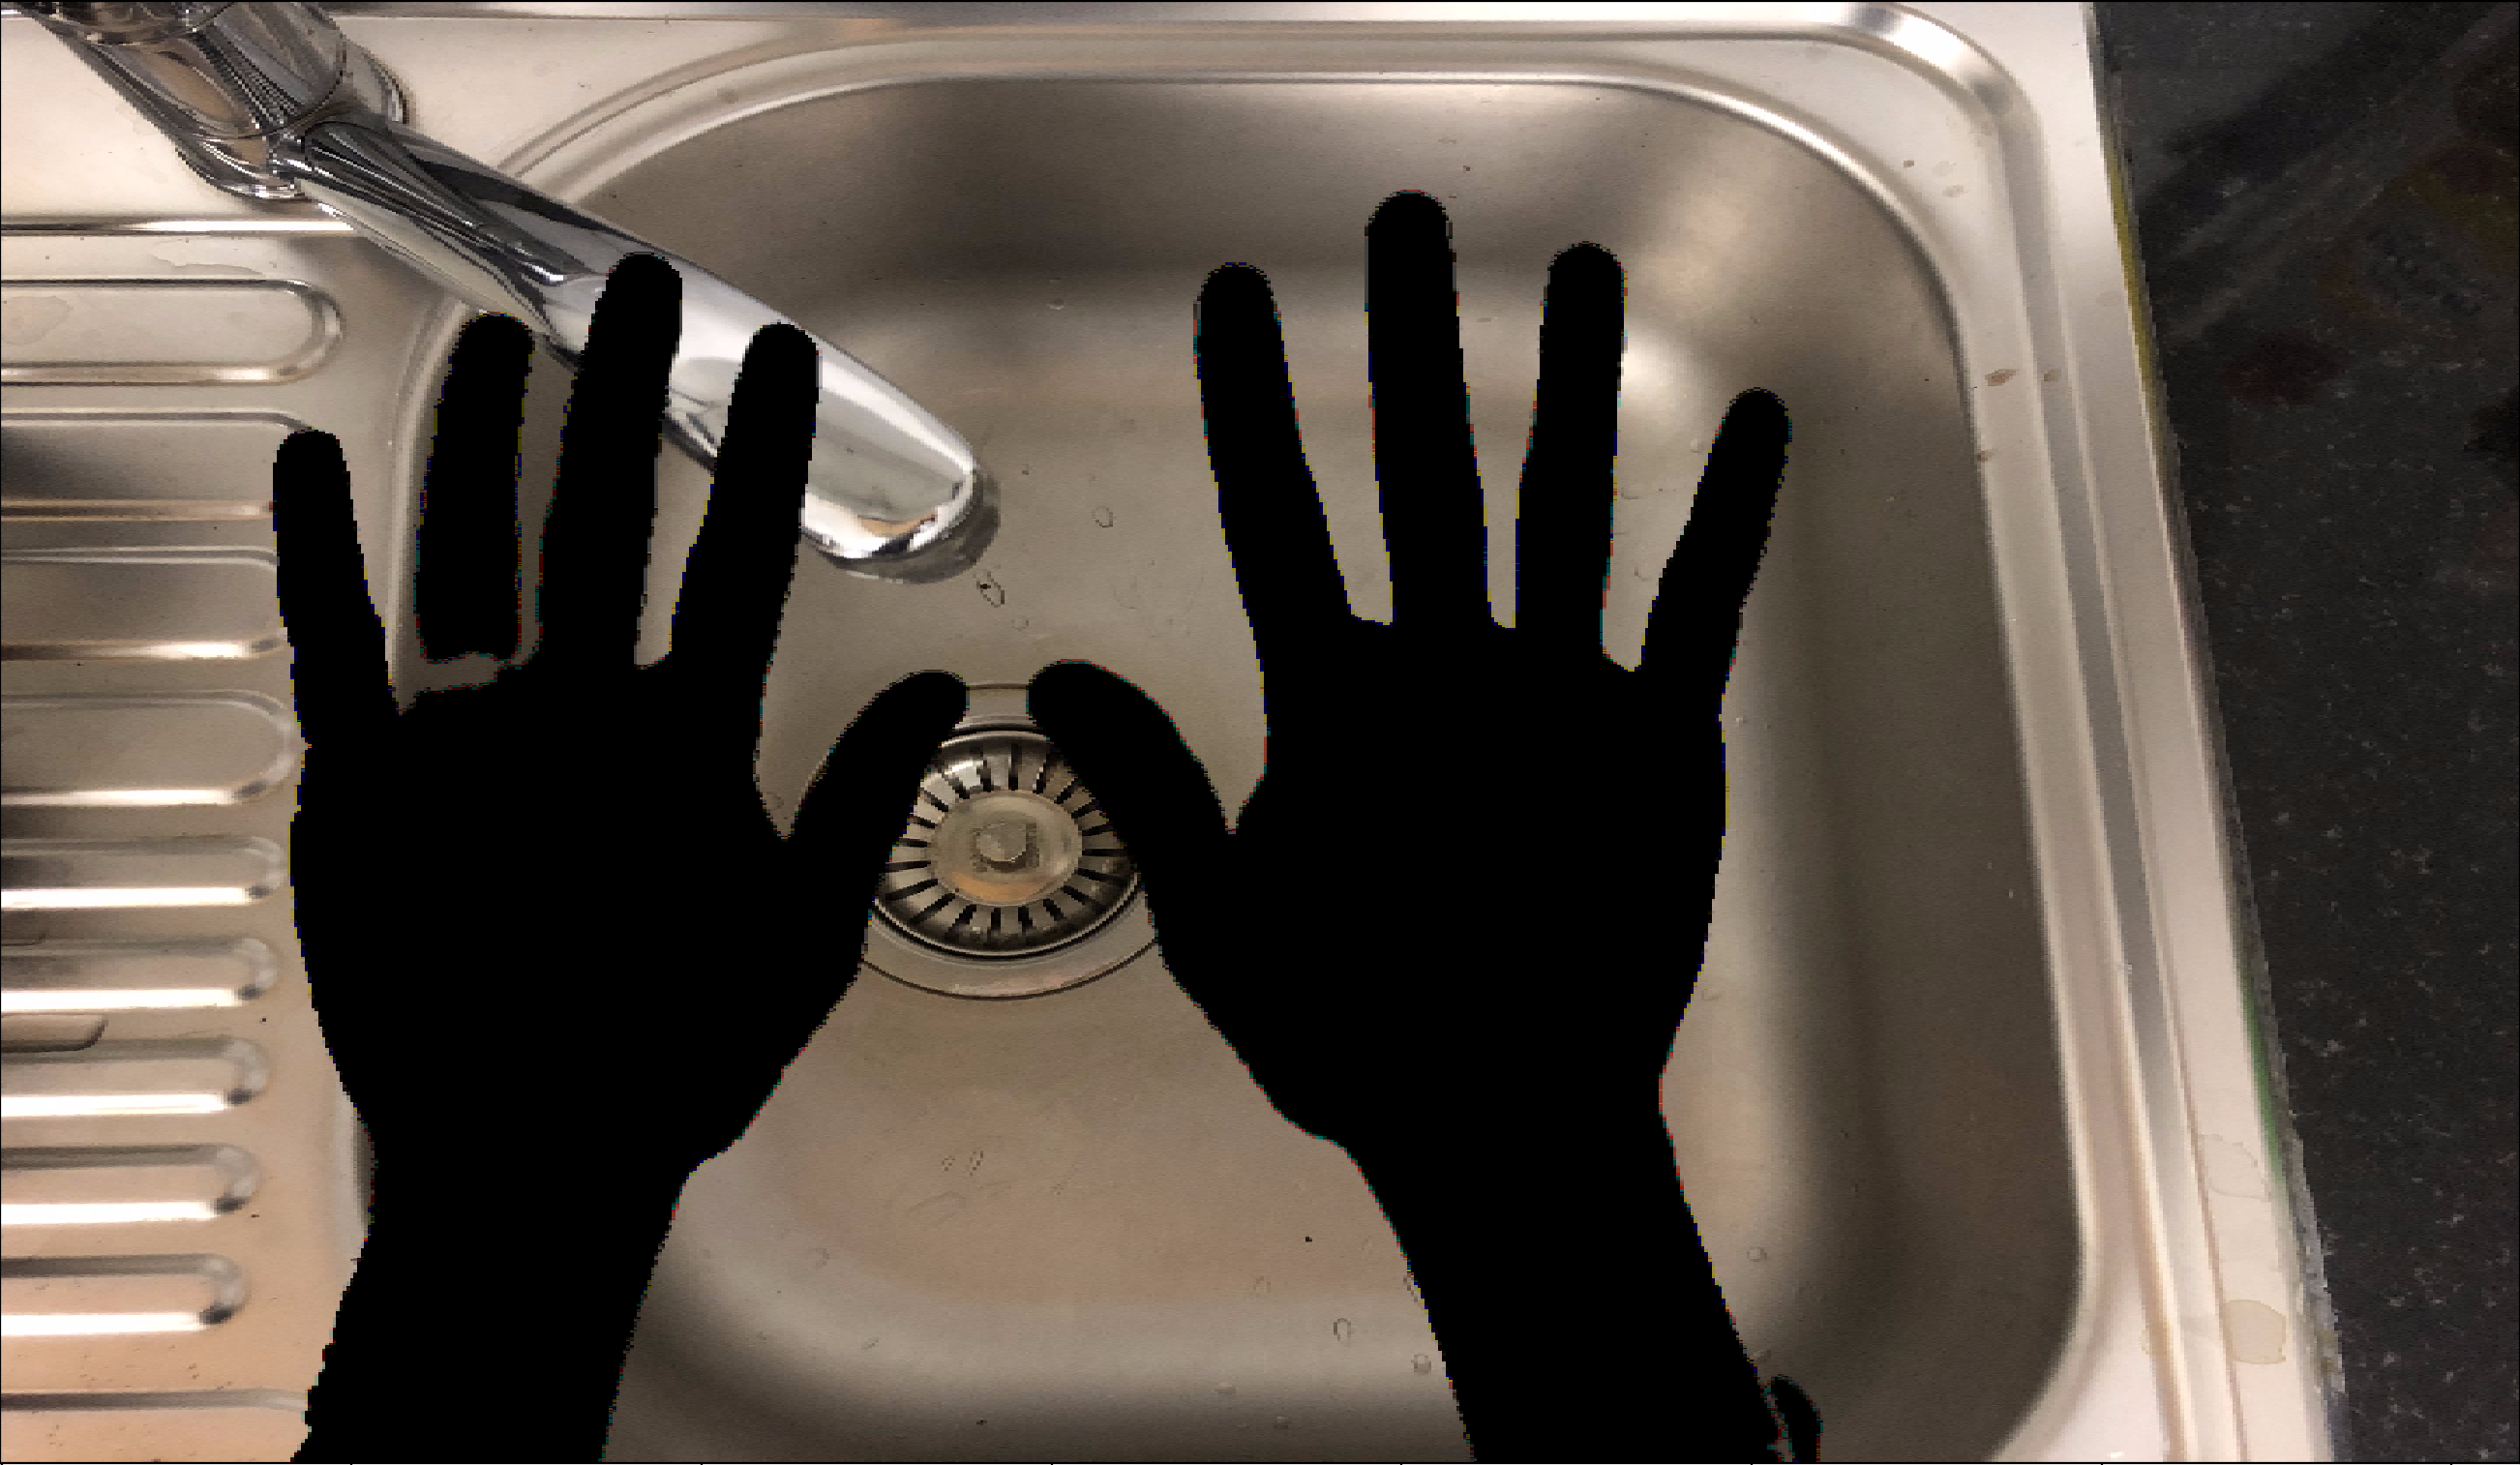
\includegraphics[width=114pt]{../img/handspipeline/5.png}
            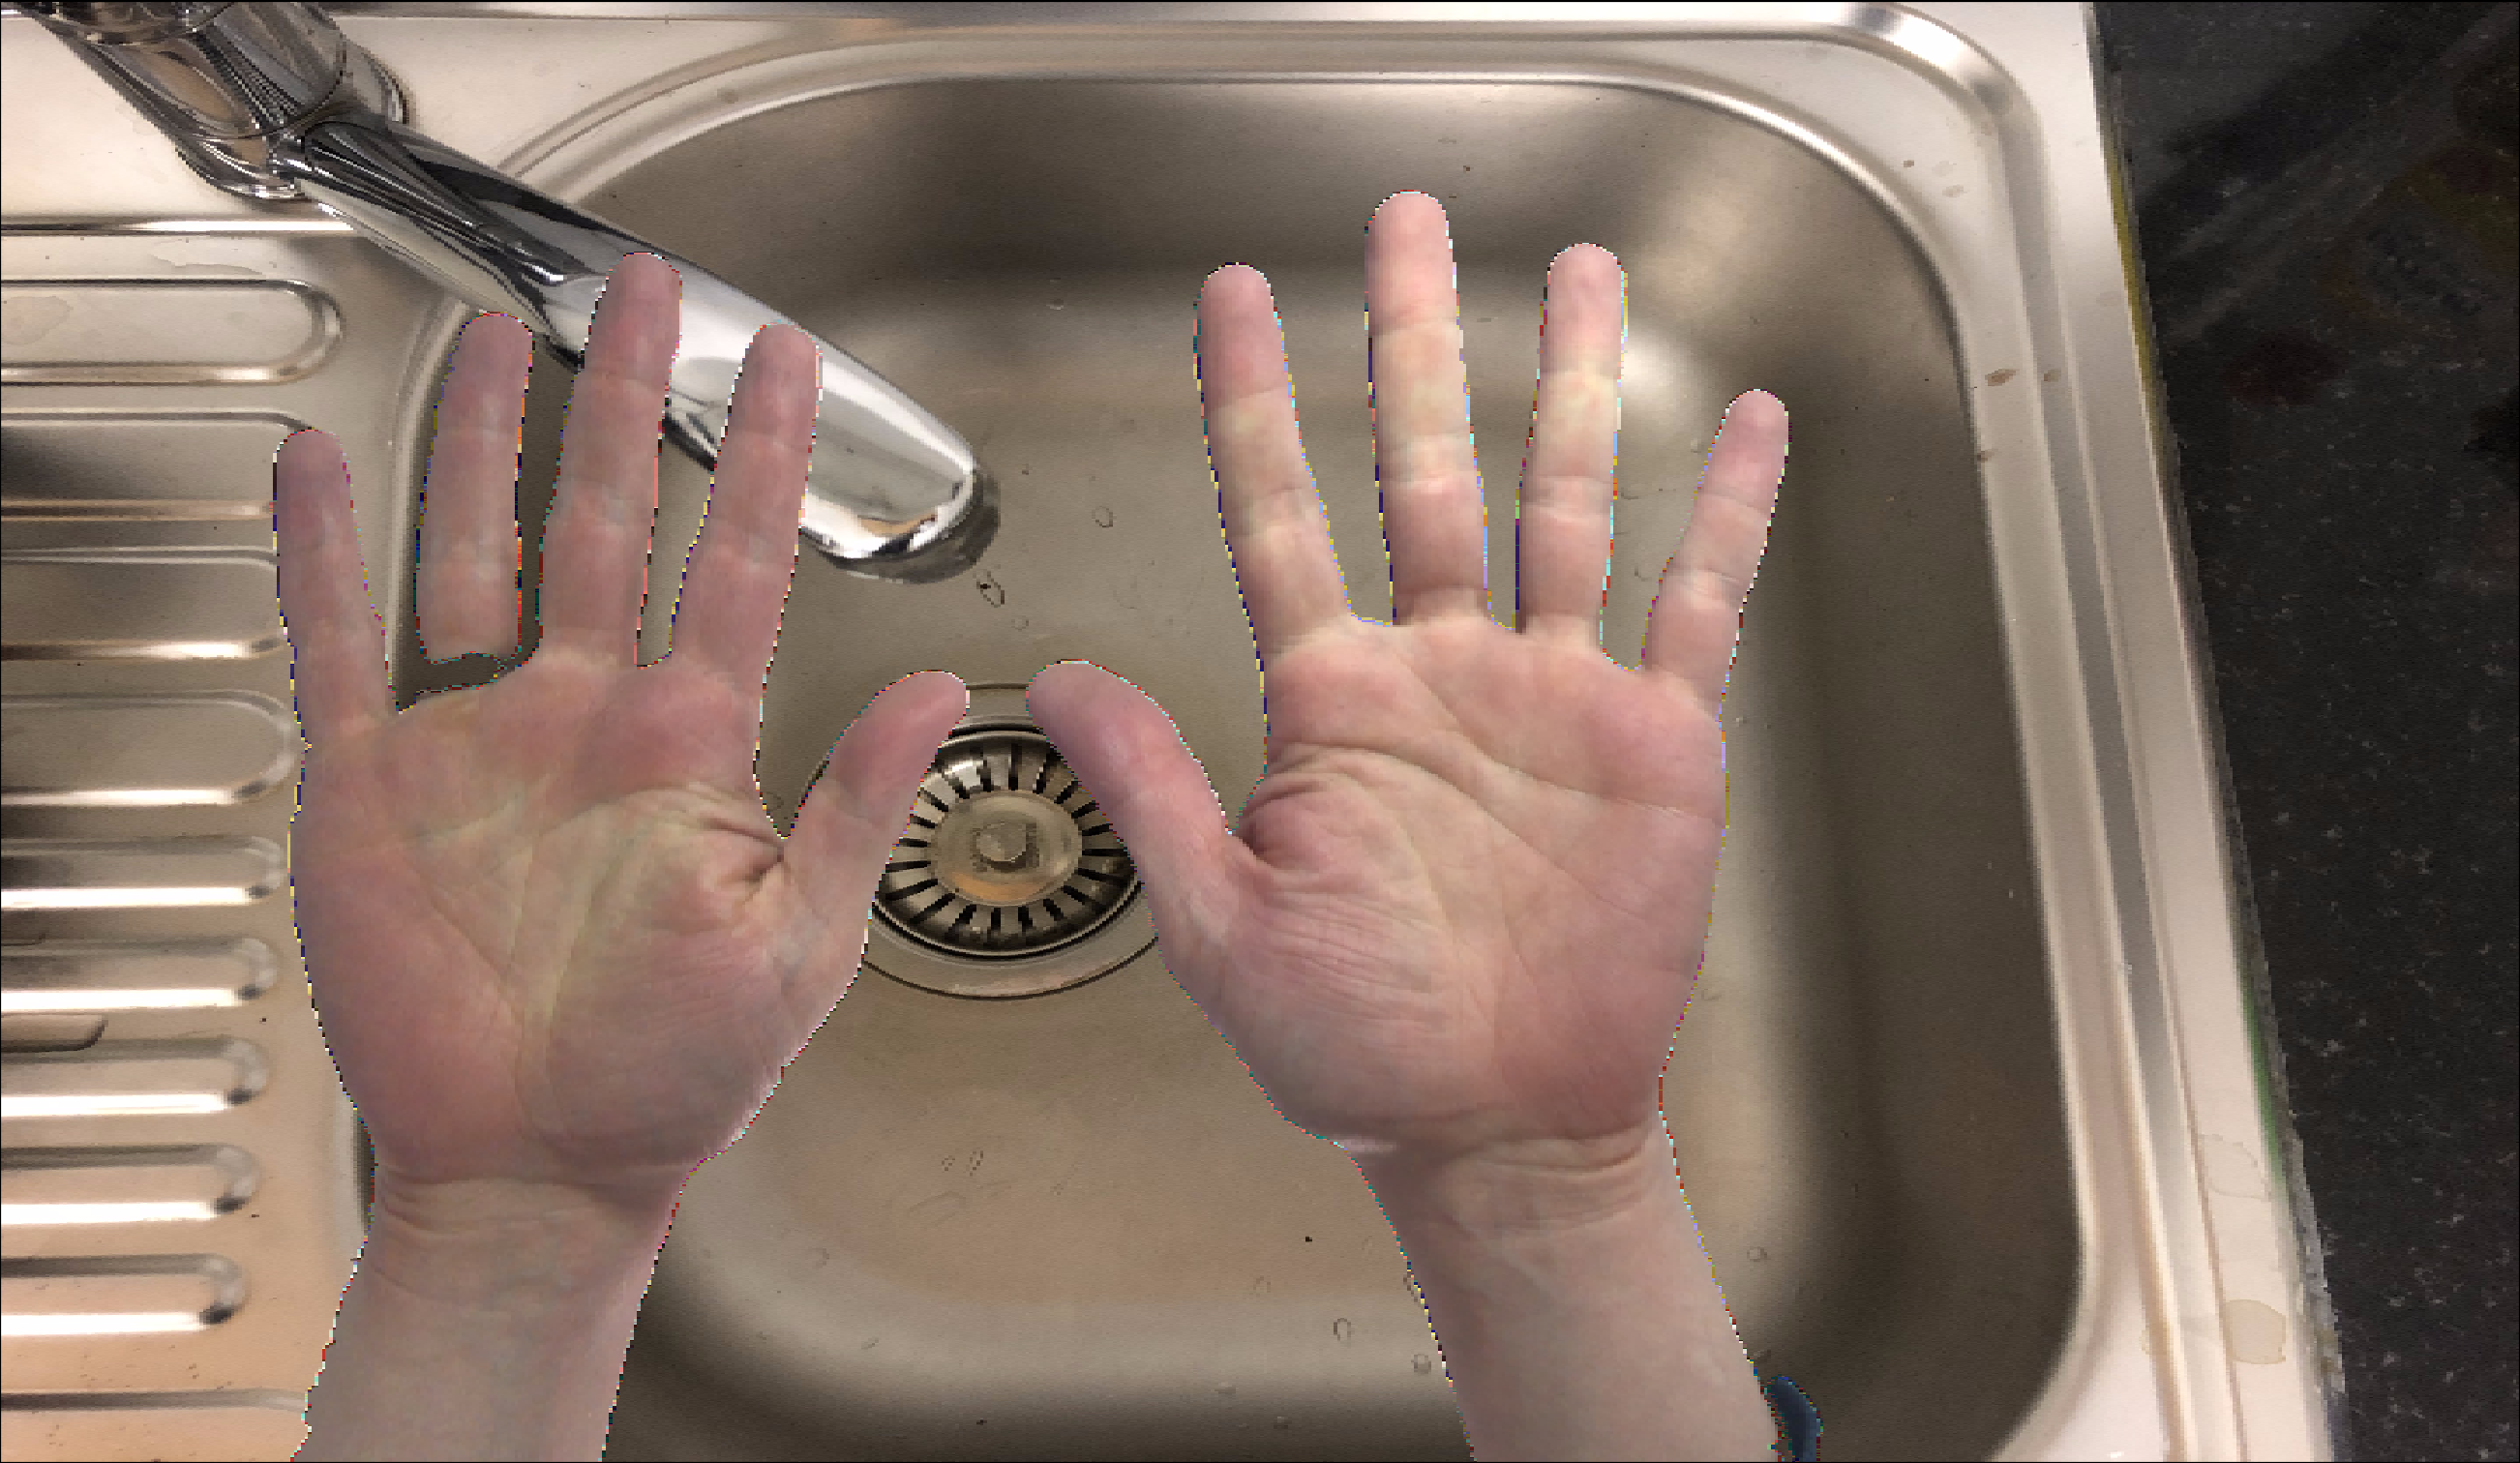
\includegraphics[width=114pt]{../img/handspipeline/6.png}
            \caption{Top left to bottom right: $HAND$, $ROI$, $BACKGROUND$, $Y_{foreground}$, $Y_{background}$, $OUTPUT$. Images \copyright \space Glanta DAC}
            \label{fig:handlogicimg}
        \end{figure}

        \subsubsection{Transformation}
        A transformation can be used as a data augmentation strategy, but some caution needs to be used. As an example, flipping figure \ref{fig:flipped_example} will also change its class, since there is a corresponding pose for the left and right hands. 

        \begin{figure}[h]
            \centering
            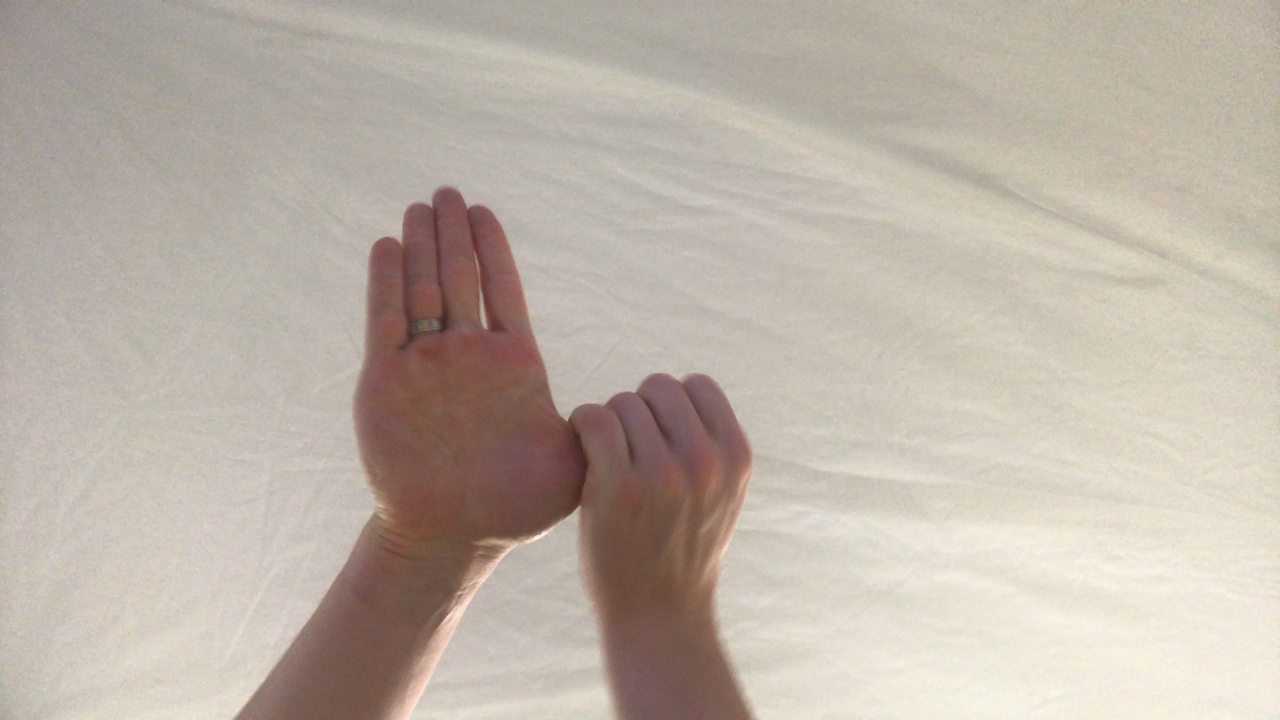
\includegraphics[height=100pt]{../img/flipped_example.png}
            \caption{\copyright \space Glanta DAC}
            \label{fig:flipped_example}
        \end{figure}

        \paragraph{Affine transformation}
        Affine transformations were applied to the hand to warp the shape of the hands, given that human hands can come in many shapes and sizes, as well as orientations in a camera. An example can be seen in figure \ref{fig:affine_example}.

        \begin{figure}[h]
            \centering
            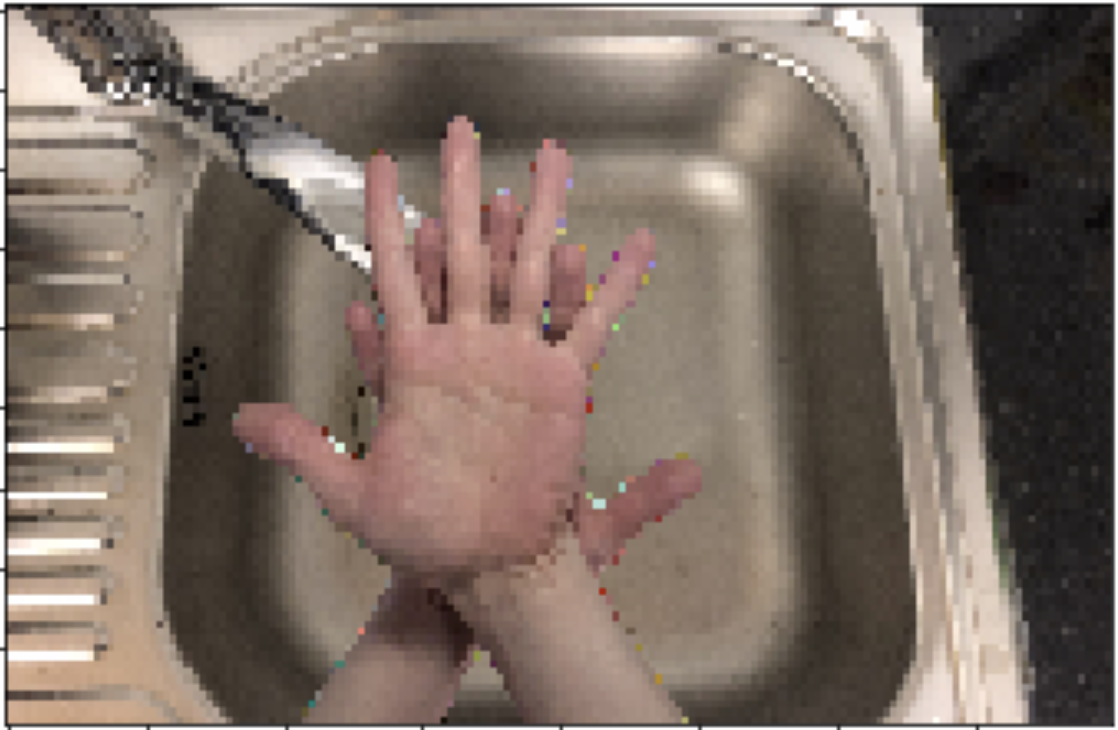
\includegraphics[height=100pt]{../img/affine/0.png}
            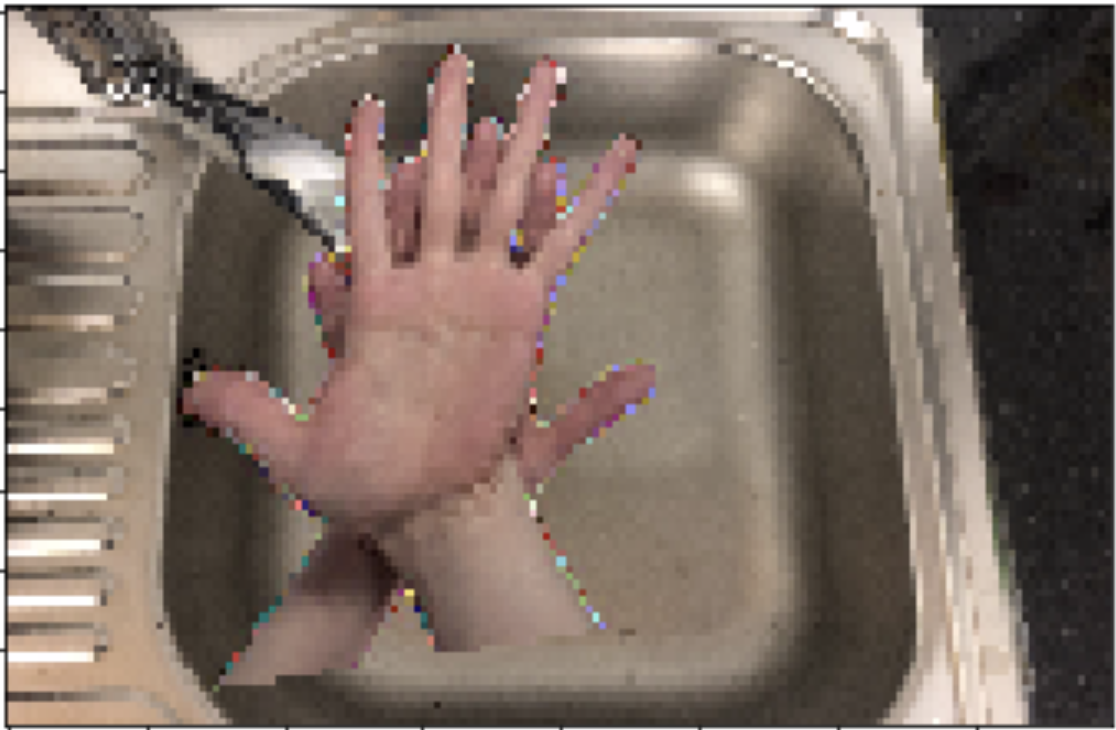
\includegraphics[height=100pt]{../img/affine/1.png}
            \caption{Affine Transformation - \copyright \space Glanta DAC}
            \label{fig:affine_example}
        \end{figure}

\section{Training}
    \subsection{Architecture}
    It has been shown that reusing a pre-trained neural network can produce state-of-the-art results on a given problem even with a small amount of training data (\cite{Razavian_2014_CVPR_Workshops}), that is therefore the strategy that was pursued in this project. A pre-trained VGG16 network was chosen, trained on ImageNet (\cite{imagenet_cvpr09}). Given that the dataset was small, only the fully-connected layers were trained. Below is the Python code that was used to train this VGG16 model. The data was split 70/30 between training and validating respectively.
    \begin{lstlisting}[style=PythonStyle]
vgg_conv = VGG16(weights='imagenet', include_top=False, input_shape=(img_rows, img_cols, 3))
for layer in vgg_conv.layers:
    layer.trainable = False
x = vgg_conv.output
x = Flatten()(x)
x = Dense(4096, activation='relu')(x)
x = Dense(4096, activation='relu')(x)
x = Dense(1000, activation='relu')(x)
predictions = Dense(20, activation='softmax', name='dd_output')(x)
model = keras.models.Model(inputs=vgg_conv.input, outputs=predictions)
opt = keras.optimizers.SGD(lr=0.01, decay=1e-6, momentum=0.9, nesterov=True)
model.compile(optimizer=opt, loss='categorical_crossentropy', metrics=['accuracy'])
model.fit(x_train, y_train, batch_size=128, epochs=20, verbose=1, validation_data=(x_test, y_test))
score = model.evaluate(x_test, y_test, verbose=0)\end{lstlisting}

    \subsection{Deployment}
    My fellow intern, Gaurav was working on finding a way to connect the Realsense camera to the NCS to perform live inference. The final stage of this project would have involved testing in a real-world scenario where the NCS is inferring live, based on the feed of the camera. Unfortunately, we had to move on to the next project, so this was never achieved.

    \subsection{Results}
    Overall, an accuracy of 60\% was achieved from the trained neural network based on a separate verification test set, but since it was not possible to connect a Realsense camera during development, it was not possible to evaluate real-world performance.

\section{Conclusion}
    \subsection{Learning Outcomes}
        \subsubsection{Improve my skills in programme design}
            \paragraph{Third party libraries} I learned how using a third party library like NumPy can dramatically improve the efficiency of a Python programme.
        \subsubsection{Enhance my time management skills}
            \paragraph{Working with a remote server} I learned how using a compression tool like 7-Zip can save time when uploading a large file to a remote server over the internet.
        \subsubsection{Other}
            \paragraph{Artificial Neural Networks} I gained practical experience training a neural network, which has improved my intuition on how I should approach a problem that has the potential to be solved using an ANN.